\begin{frame}{
    Methods for fast nearest neighbor queries:
    }

\Large

%\vspace{0.15in}

\newcommand{\yes}{\cellcolor{green}yes}
\newcommand{\no}{\cellcolor{red}no}
\newcommand{\maybe}{\cellcolor{yellow}somewhat}

\begin{center}
\renewcommand{\arraystretch}{1.75}
\begin{tabular}{cccc}
\hline
%Method
& \parbox{1in}{\centering provable\\speedup}
& \parbox{1in}{\centering arbitrary\\metric}
& \parbox{1in}{\centering high\\dimensions}
\\
\hline
\hline
quadtree & \yes & \no & \no \\
$k$d-tree & \yes & \no & \maybe \\
%\hline
hashing & \yes & \no & \yes \\
%\hline
ball tree & \no & \yes & \maybe \\
\textbf{cover tree} & \yes & \yes & \yes \\
\hline
\end{tabular}

\vspace{-0.1in}
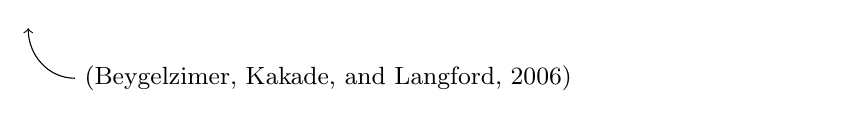
\begin{tikzpicture}
%\node (a) {\small (Beygelzimer \emph{et. al.}, 2006)};
\node (a) {\small (Beygelzimer, Kakade, and Langford, 2006)};
\node at (2.5in,0) {};
\draw[->] (a) to[out=180,in=270]  (-1.5in,0.25in);
\end{tikzpicture}
\end{center}
\end{frame}

%%%%%%%%%%%%%%%%%%%%%%%%%%%%%%%%%%%%%%%%%%%%%%%%%%%%%%%%%%%%%%%%%%%%%%%%%%%%%%%%

\begin{frame}{Other uses of cover trees}

\Large
Any learning algorithm that cares about distance can be made faster using cover trees.
\vspace{0.15in}

Examples:
\begin{itemize}
\item $k$-nearest neighbor
\item Support vector machines (Segata and Blanzieri, 2010)
\item Dimensionality reduction (Lisitsyn \emph{et. al.}, 2010)
%\item Clustering
\item Reinforcement learning (Tziortziotis \emph{et. al.}, 2014)
\end{itemize}

\end{frame}
